\documentclass[12pt,twoside]{report}
\usepackage{graphicx}
\usepackage{alphalph}
\usepackage{subcaption}
\usepackage[a5paper,margin=1cm]{geometry}
\renewcommand*{\thesubfigure}{(\arabic{subfigure})}
\begin{document}
\begin{figure}
\centering
\begin{subfigure}[b]{0.20\textwidth}
\centering

\includegraphics[width=\textwidth]{../trajectories/173.png}
\caption{Id:173}
\end{subfigure}
\begin{subfigure}[b]{0.20\textwidth}
\centering

\includegraphics[width=\textwidth]{../trajectories/543.png}
\caption{Id:543}
\end{subfigure}
\begin{subfigure}[b]{0.20\textwidth}
\centering

\includegraphics[width=\textwidth]{../trajectories/577.png}
\caption{Id:577}
\end{subfigure}
\begin{subfigure}[b]{0.20\textwidth}
\centering
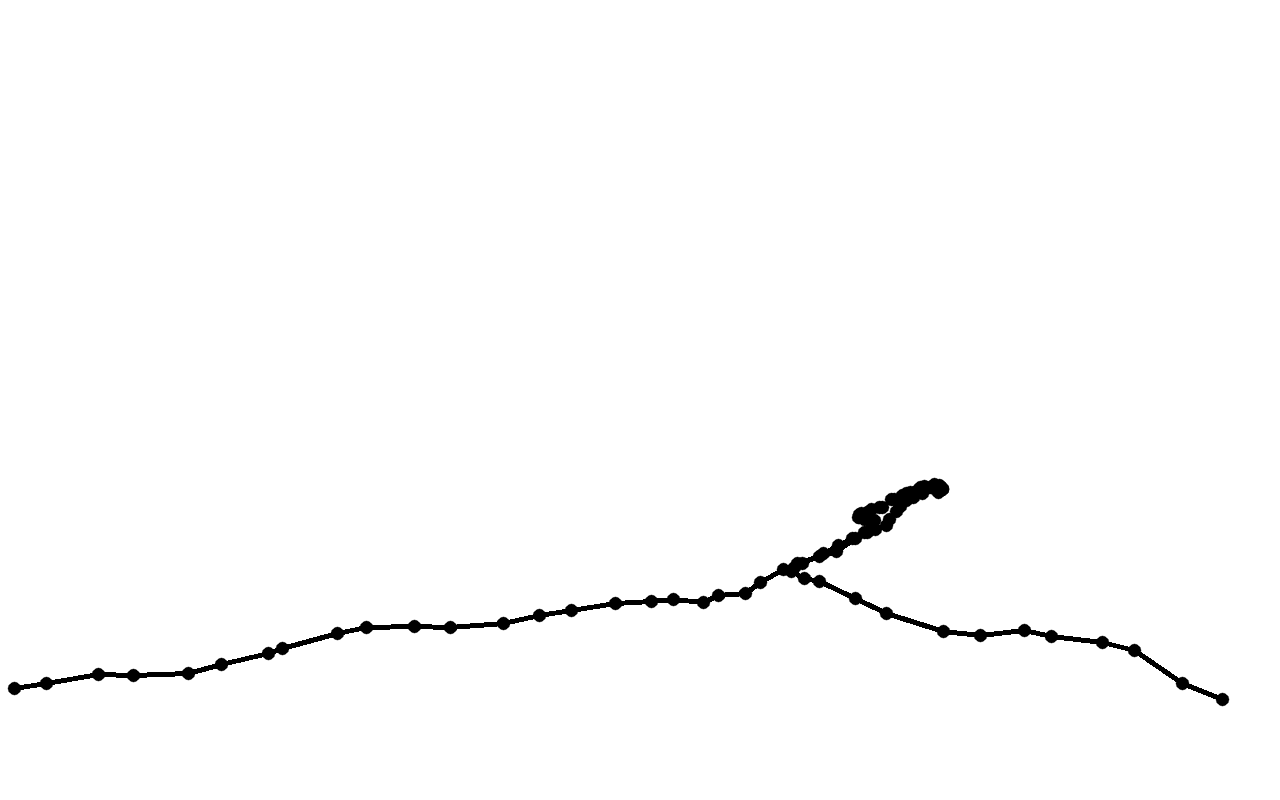
\includegraphics[width=\textwidth]{../trajectories/626.png}
\caption{Id:626}
\end{subfigure}
\begin{subfigure}[b]{0.20\textwidth}
\centering
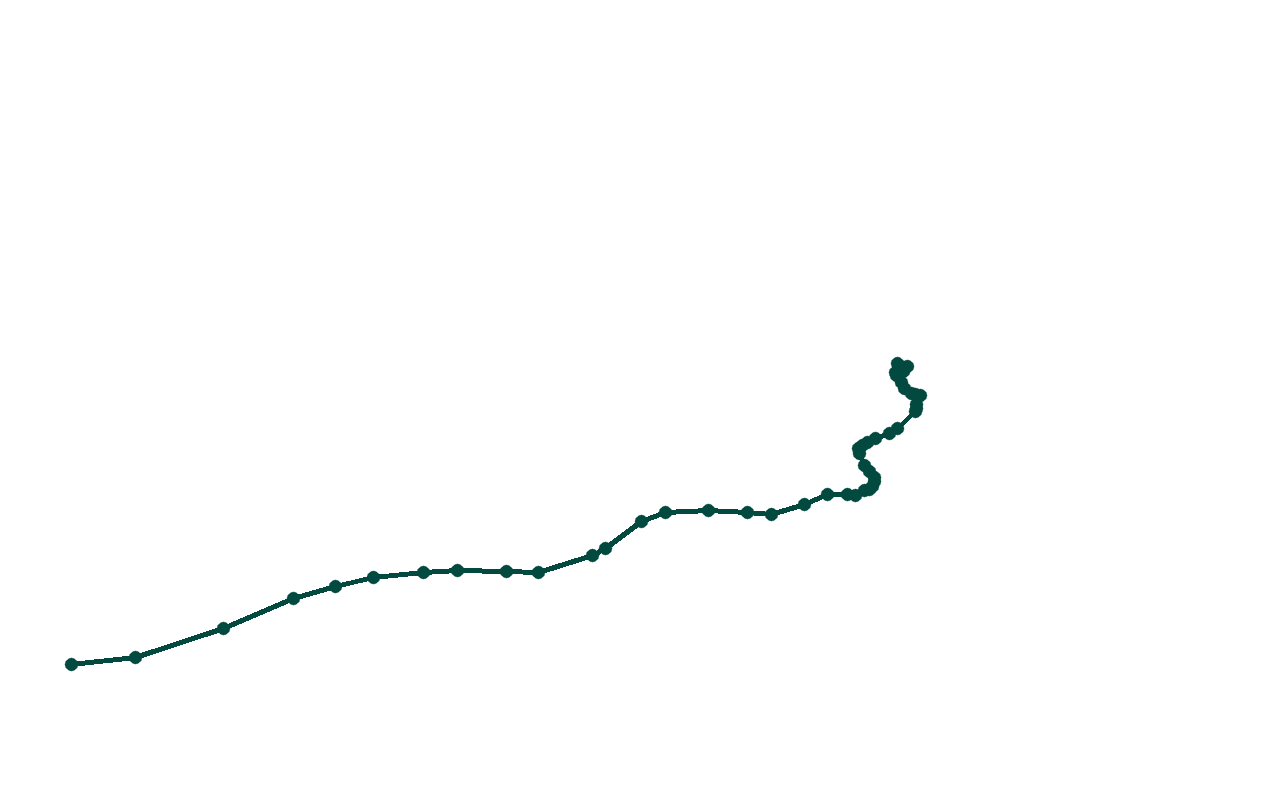
\includegraphics[width=\textwidth]{../trajectories/685.png}
\caption{Id:685}
\end{subfigure}
\begin{subfigure}[b]{0.20\textwidth}
\centering

\includegraphics[width=\textwidth]{../trajectories/776.png}
\caption{Id:776}
\end{subfigure}
\begin{subfigure}[b]{0.20\textwidth}
\centering

\includegraphics[width=\textwidth]{../trajectories/814.png}
\caption{Id:814}
\end{subfigure}
\begin{subfigure}[b]{0.20\textwidth}
\centering

\includegraphics[width=\textwidth]{../trajectories/845.png}
\caption{Id:845}
\end{subfigure}
\begin{subfigure}[b]{0.20\textwidth}
\centering

\includegraphics[width=\textwidth]{../trajectories/911.png}
\caption{Id:911}
\end{subfigure}
\begin{subfigure}[b]{0.20\textwidth}
\centering
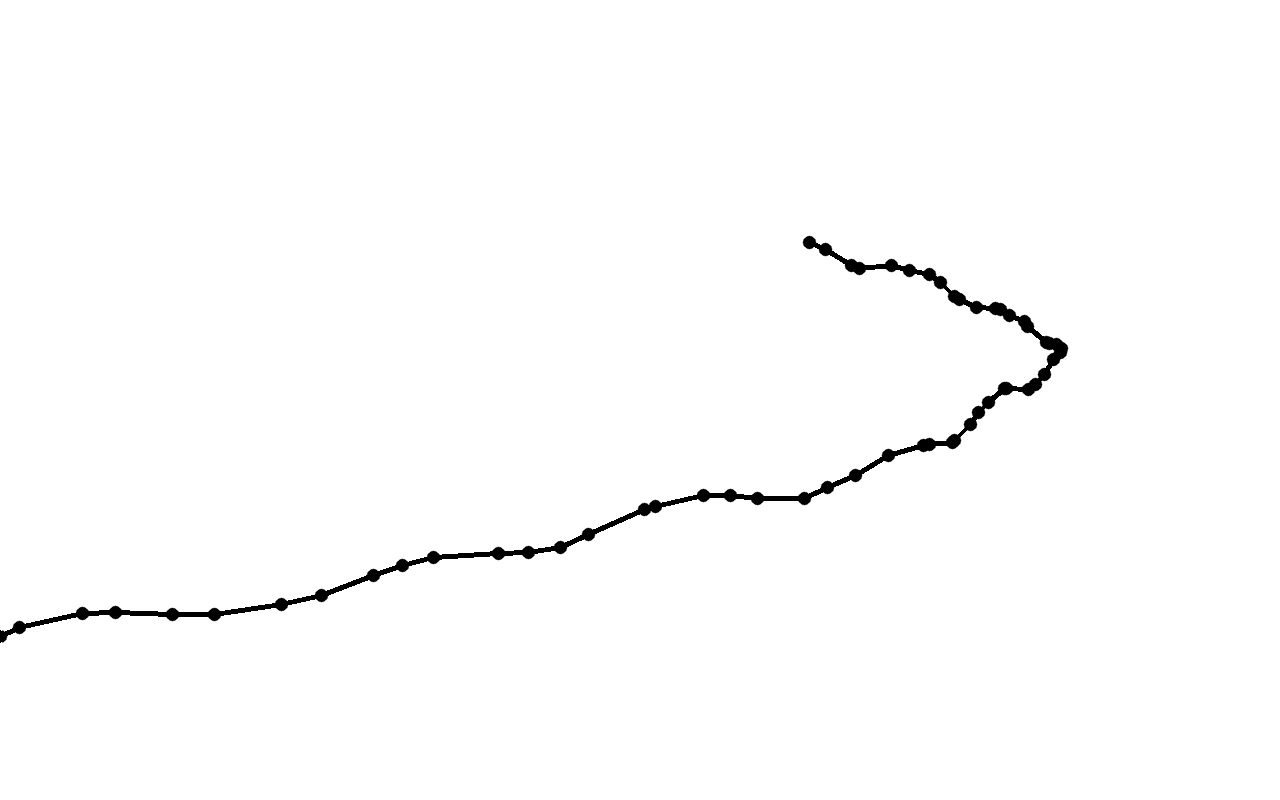
\includegraphics[width=\textwidth]{../trajectories/962.png}
\caption{Id:962}
\end{subfigure}
\begin{subfigure}[b]{0.20\textwidth}
\centering

\includegraphics[width=\textwidth]{../trajectories/980.png}
\caption{Id:980}
\end{subfigure}
\begin{subfigure}[b]{0.20\textwidth}
\centering

\includegraphics[width=\textwidth]{../trajectories/989.png}
\caption{Id:989}
\end{subfigure}
\end{figure}
\end{document}